\documentclass[12pt, a4paper]{article} 

\usepackage{fontspec}
\usepackage{polyglossia}
\setdefaultlanguage{russian}
\setotherlanguage{english}
\newfontfamily\cyrillicfont{Arial}

\usepackage{hyperref}
\usepackage{amsmath,amsfonts,amssymb,amsthm,mathtools}  

\usepackage{graphicx}
\usepackage{tikzsymbols}


\renewcommand{\section}{\Smiley{ }}

\title{Задание 1. Версия 2}
\author{Алиса Жильцова}


\begin{document}

\maketitle

\section{Фактов 10 о себе}

\begin{enumerate}
\item Меня зовут Алиса - необычный факт из моей жизни;
\item Мою собаку зовут Марвин, и назвали ее в честь Марвина Бауэра ( при желании по этому же имении ее можно найти в фейсбуке);
\item Я люблю математику во всех ( или почте во всех) её проявлениях, но я не люблю об этом говорить, однако считаю своим долгом об этом все же сказать;
\item Je parle français, немного хуже I speak english и совсем чуть-чуть (только учусь) ich spreche Deutsch;
\item Я люблю кино. Сильно люблю кино. А особенно ужасы, и считаю, что ужасы - это недооцененный жанр;
\item Еще больше я люблю театр. Особенно Театр на Юго-Западе. Приходите в Театр на Юго-Западе! Он правда очень крутой!
\item Люблю готовить. И люблю чай. Но чаще приходится пить кофе \Coffeecup \pot
\item Если говорить о традициях эконома, то ни разу не была ни на капустнике, ни на мероприятии после него;
\item Я часто пишу с ошибками. Наверное, вы уже заметили;
\item В детстве мечтала стать альпинисткой, но как-то не вышло \Snowman


\end{enumerate}

\section{Любимых 5 формул}

\begin{equation}
\label{f1} 
\tilde{\sigma}_{\hat{\beta}_0}^2=\frac{\left(\frac{1}{n} \cdot \sum\limits_{i=1}^n x_i^2\right)\cdot S_{\hat{u}}^2}{\sum\limits_{i=1}^n\left(x_i-\bar{x}\right)^2}\tag{\ae}
\end{equation}


\begin{equation}
\label{f2} 
\Phi(x)=\frac{2}{\sqrt{\pi}}\int\limits_0^xe^{-t^2}dt\tag{\ae\ae}
\end{equation}


\begin{equation}
\label{f3} 
f'(x_0)=\lim\limits_{x \to x_0}\frac{f\left(x_0+\Delta x\right)-f(x_0)}{\Delta x}\tag{\ae\ae\ae}
\end{equation}

\begin{equation}
\label{f4} 
\Gamma(x) = \int\limits_0^{\infty} t^{x-1} e^{-t} dt\tag{\ae\ae\ae\ae}
\end{equation}


\begin{align*}
\label{f5} 
&\begin{pmatrix}
  a_{1,1} & a_{1,2} & \cdots & a_{1,m} \\
  a_{2,1} & a_{2,2} & \cdots & a_{2,m} \\
  \vdots  & \vdots  & \ddots & \vdots  \\
  a_{l,1} & a_{l,2} & \cdots & a_{l,m}
 \end{pmatrix} \times \begin{pmatrix}
  b_{1,1} & b_{1,2} & \cdots & b_{1,n} \\
  b_{2,1} & b_{2,2} & \cdots & b_{2,n} \\
  \vdots  & \vdots  & \ddots & \vdots  \\
  b_{m,1} & b_{m,2} & \cdots & b_{m,n}
 \end{pmatrix}=\\
  & =\begin{pmatrix}
  \sum\limits_{i=1}^m a_{1,i}b_{i,1} & \sum\limits_{i=1}^m a_{1,i}b_{i,2} & \cdots & \sum\limits_{i=1}^m a_{1,i}b_{i,n} \\
  \sum\limits_{i=1}^m a_{2,i}b_{i,1} & \sum\limits_{i=1}^m a_{2,i}b_{i,2} & \cdots & \sum\limits_{i=1}^m a_{2,i}b_{i,n} \\
  \vdots  & \vdots  & \ddots & \vdots  \\
  \sum\limits_{i=1}^m a_{l,i}b_{i,1} & \sum\limits_{i=1}^m a_{l,i}b_{i,2} & \cdots & \sum\limits_{i=1}^m a_{l,i}b_{i,n} \end{pmatrix}\tag{\ae\ae\ae\ae\ae}
\end{align*}

\begin{multline*}
\label{f6} 
 \Delta Q_{(p)}=\sum\limits_{i=1}^n q_{1i}\cdot p_{0i} - \sum\limits_{i=1}^n q_{0i}\cdot p_{0i}=\\
  =\sum\limits_{i=1}^n w_{1i}\cdot T_{1i} - \sum\limits_{i=1}^n w_{0i}\cdot T_{1i}+\\
 +\left(\frac{\sum\limits_{i=1}^n w_{0i} \cdot T_{1i}}{\sum\limits_{i=1}^n T_{1i}} - \frac{\sum\limits_{i=1}^n w_{0i}\cdot T_{0i}}{\sum\limits_{i=1}^n T_{0i}}\right)\cdot\sum\limits_{i=1}^nT_{1i}+\\
 +\left(\sum\limits_{i=1}^n T_{1i} - \sum\limits_{i=1}^n T_{0i}\right)\cdot\bar w_0 \tag{\ae\ae\ae\ae\ae\ae}
 \end{multline*}

\section{Пояснения к формулам}


Формула \ref{f1}  - первая формула, которая пришла мне в голову, когда я увидела задание. \Smiley По необъяснимым причинам мне  просто нравится её выводить ( даже больше чем расставлять смайлики в \LaTeX ). Формула  \ref{f2} полюбилась за время многочисленных встреч с ней в курсе теор.вера и мат.стата. А вот с формулой  \ref{f3}  вообще немного странная история... она у меня с Папасом ассоциируется. Формула \ref{f5} просто прикольная и большая ( здесь большая получилась). Формула \ref{f4} - последняя, которую я написала. Почему бы и нет? Чирский, например, считает Гамма-функцию чуть ли не одним из самых значимых открытий математики ( он как-то это обсуждал с Поповым А.Ю. после нашей лекции).

P.S. На самом деле формула \ref{f4} была не последней. Последняя формула - \ref{f6},которая полюбилась за то, что раскладывать изменение стоимости выпуска по факторам просто забавно.

\section{Нелюбимые формулы}


Таких нет. \Smiley 

\section{Фотка}


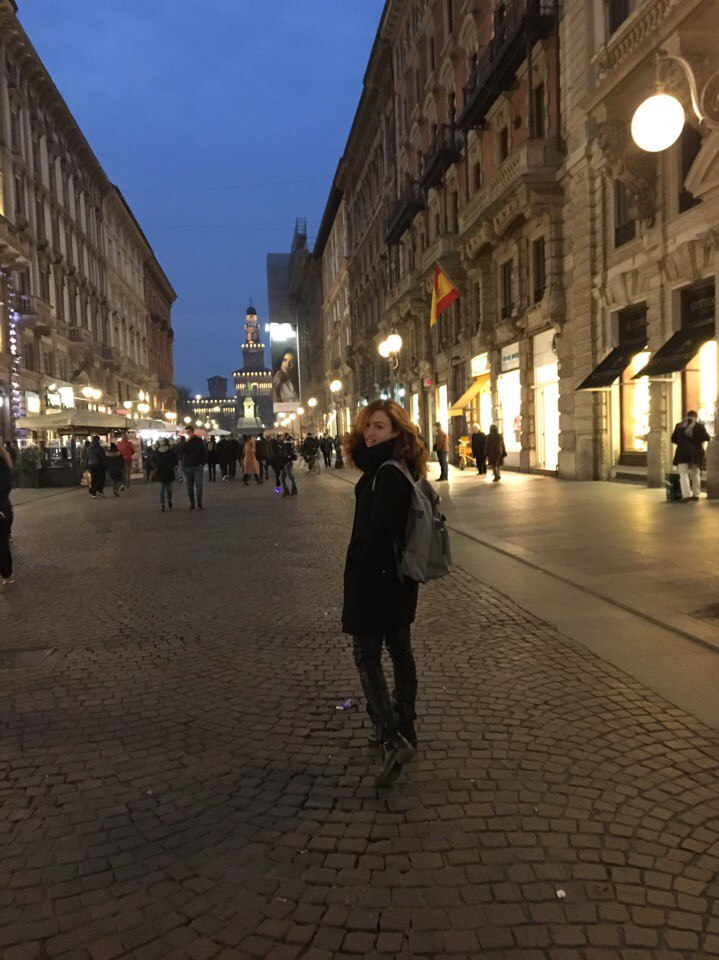
\includegraphics[width=10 cm]{alisa.jpg}

\end{document}
